\thispagestyle{empty}
\refstepcounter{dummy}
\addcontentsline{toc}{chapter}{\tocEntry{Paper I}}
%*******************************************************
\topskip0pt
\vspace*{\fill}
\begin{flushright}
\Huge{\textbf{Paper I}}
\end{flushright}

\Large{
\textsc{Four-Component Relativistic Calculations in Solution with the
Polarizable Continuum Model of Solvation: Theory,
Implementation, and Application to the
Group 16 Dihydrides
\ce{H2X} (\ce{X} = \ce{O}, \ce{S}, \ce{Se}, \ce{Te},
    \ce{Po})}
\\
\textbf{R. Di Remigio}, R. Bast, L. Frediani, and T. Saue
\\
\textit{J. Phys. Chem. A}, \textrm{2015}, \textbf{119}, 5061--5077
}
\vspace*{\fill}

\includepdf[pages=-]{papers/relapcm.pdf}

\thispagestyle{empty}
\refstepcounter{dummy}
\addcontentsline{toc}{chapter}{\tocEntry{Paper II}}
%*******************************************************
\topskip0pt
\vspace*{\fill}
\begin{flushright}
\Huge{\textbf{Paper II}}
\end{flushright}

\Large{
\textsc{
Wavelet Formulation of the Polarizable Continuum Model. II. Use of Piecewise
Bilinear Boundary Elements
}
\\
M. Bugeanu, \textbf{R. Di Remigio}, K. Mozgawa, S. S. Reine, H.
Harbrecht,  and L. Frediani
\\
\textit{Phys. Chem. Chem. Phys.}, \textrm{2015}, \textbf{17},
31566--31581
}
\vspace*{\fill}

\includepdf[pages=-]{papers/wemlin.pdf}

\thispagestyle{empty}
\refstepcounter{dummy}
\addcontentsline{toc}{chapter}{\tocEntry{Paper III}}
%*******************************************************
\topskip0pt
\vspace*{\fill}
\begin{flushright}
\Huge{\textbf{Paper III}}
\end{flushright}

\Large{
\textsc{
    A Polarizable Continuum Model for Molecules at Spherical
    Diffuse Interfaces
}
\\
    \textbf{R. Di Remigio}, K. Mozgawa, H. Cao, V. Weijo, and L.
    Frediani
\\
    \textit{J. Chem. Phys.}, \textrm{2016}, \textbf{144}, 124103
}
\vspace*{\fill}

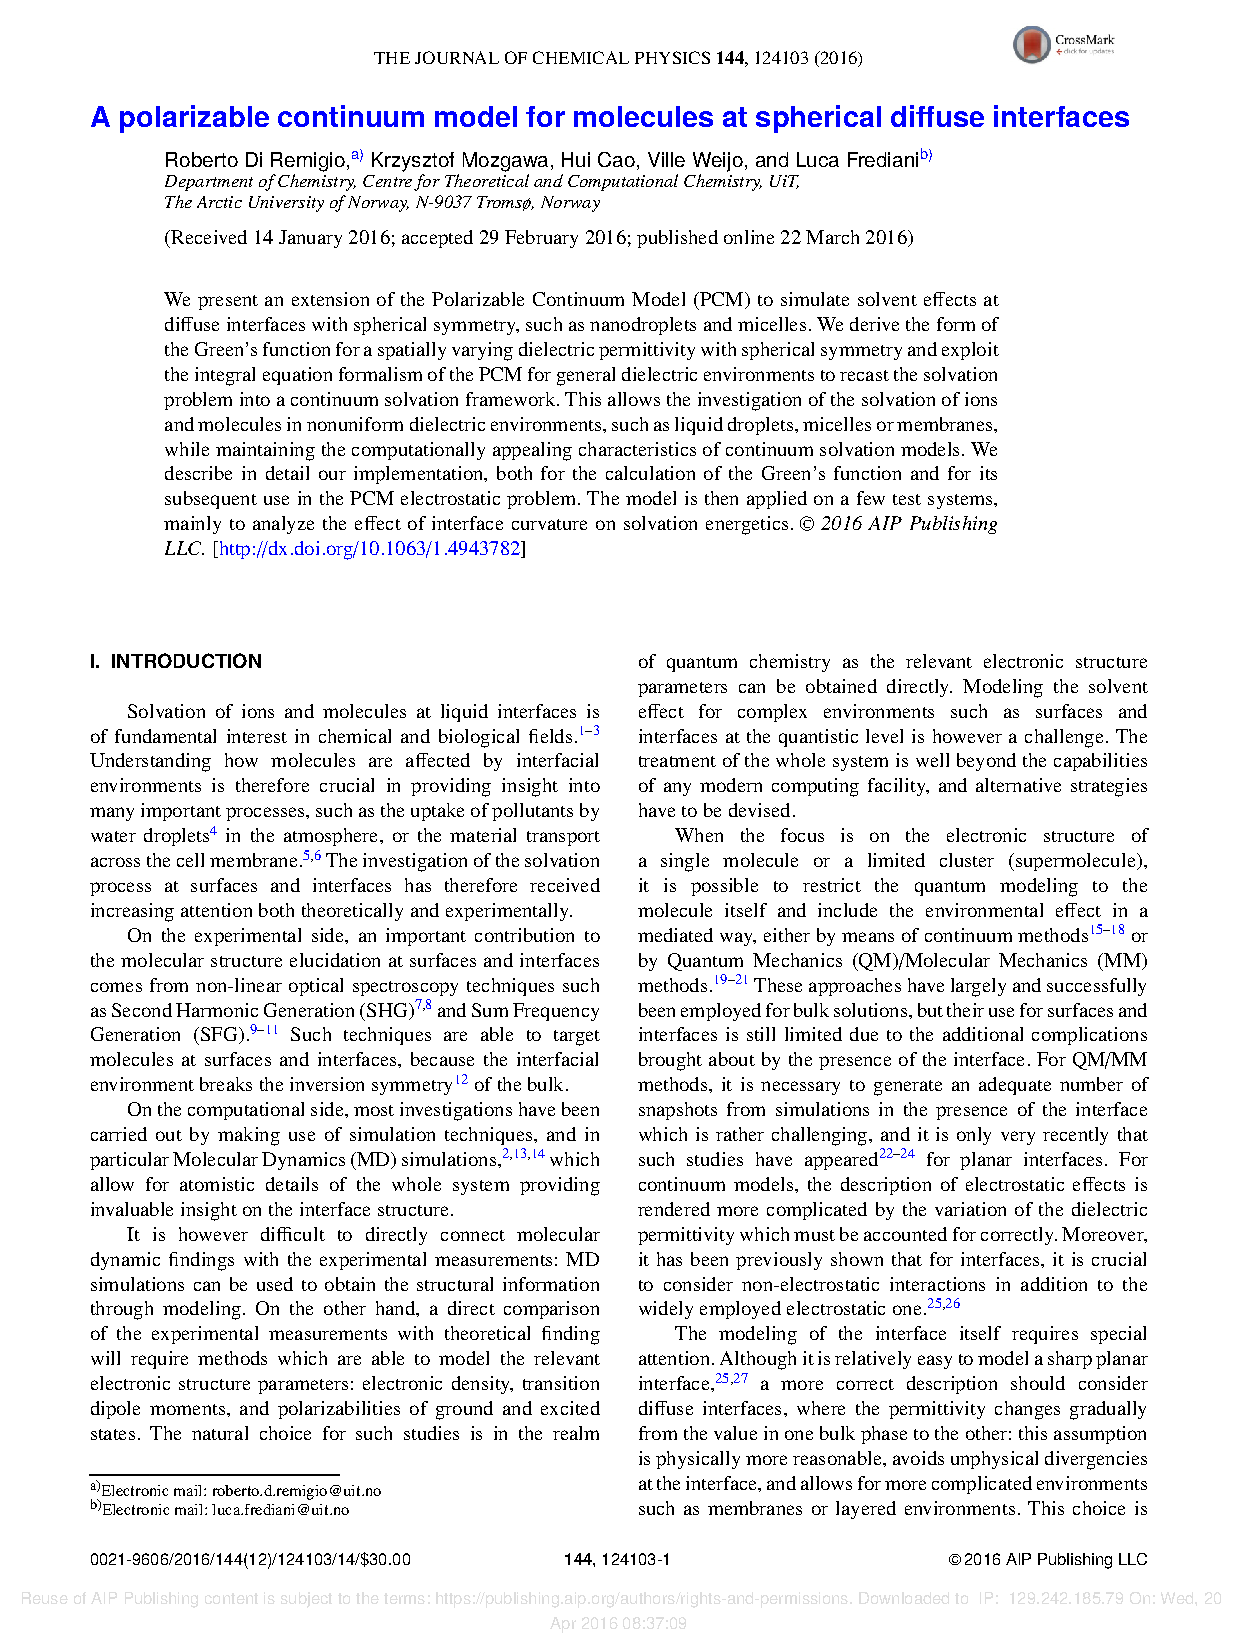
\includepdf[pages=-]{papers/spherical.pdf}

\thispagestyle{empty}
\refstepcounter{dummy}
\addcontentsline{toc}{chapter}{\tocEntry{Paper IV}}
%*******************************************************
\topskip0pt
\vspace*{\fill}
\begin{flushright}
\Huge{\textbf{Paper IV}}
\end{flushright}

\Large{
\textsc{
    Four-Component Relativistic Density Functional Theory with the
    Polarizable Continuum Model: Application to EPR Parameters
    and Paramagnetic NMR Shifts
}
\\
  \textbf{R. Di Remigio}, M. Repisky, S. Komorovsky, P. Hrobarik, L.
  Frediani, and K. Ruud
\\
  submitted for publication to \textit{Mol. Phys.}
}
\vspace*{\fill}

%\includepdf[pages=-]{papers/pcmepr.pdf}

\thispagestyle{empty}
\refstepcounter{dummy}
\addcontentsline{toc}{chapter}{\tocEntry{Paper V}}
%*******************************************************
\topskip0pt
\vspace*{\fill}
\begin{flushright}
\Huge{\textbf{Paper V}}
\end{flushright}

\Large{
\textsc{
    Open-ended formulation of self-consistent field response theory with
    the polarizable continuum model for solvation
}
\\
    \textbf{R. Di Remigio}, M. T. P. Beerepoot, Y. Cornaton, M. Ringholm,
    A. H. S. Steindal, K. Ruud, and L. Frediani
\\
    In preparation for submission to \textit{Phys. Chem. Chem. Phys.}
}
\vspace*{\fill}

%\includepdf[pages=-]{papers/pcmopenrsp.pdf}

\thispagestyle{empty}
\refstepcounter{dummy}
\addcontentsline{toc}{chapter}{\tocEntry{Paper VI}}
%*******************************************************
\topskip0pt
\vspace*{\fill}
\begin{flushright}
\Huge{\textbf{Paper VI}}
\end{flushright}

\Large{
\textsc{
  PCMSolver: an Application Programming Interface
  for the Polarizable Continuum Model
}
\\
    \textbf{R. Di Remigio}, T. D. Crawford, and L. Frediani
\\
  Accepted for publication in the proceedings of the
  \emph{Producing High Performance and Sustainable Software for
  Molecular Simulation} workshop held at the 2015 Supercomputing
  Conference
}
\vspace*{\fill}

\includepdf[pages=-]{papers/SC15.pdf}

